\subsection{Спектрохимический ряд лигандов с позиций метода молекулярных орбиталей}

Одним из главных достоинств ММО в применении к комплексам является возможность обьяснения спектрохимического ряда лигандов. Для этого нужно принять во внимание пи-взаимодействие между несвязывающими молекулярными орбиталями с атомными орбиталями лигандов, имеющих симметрию $\pi$-типа относительно линии связи металл-лиганд. Кроме электронных пар лигандов, ориентированных в направлении сигма-связи, у них остаются по две негибридизированные р-орбитали, ориентированные перпендикулярно линии связи металл-лиганд. Эти орбитали во многом определяют энергию расщепления $\Delta_{oct}$ а, следовательно, и объясняют расположение лигандов в спектрохимическом ряду. 
\begin{figure}[H]
\centering
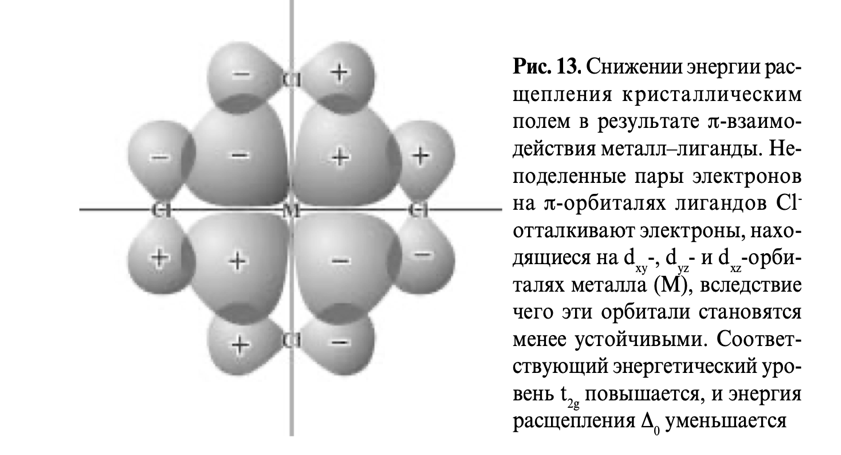
\includegraphics[scale=1.00]{images/L-M-pi.png}
\end{figure}
    Если на dxy-орбитали комплексообразователя есть электроны, то возникают силы отталкивания между электронными парами лигандов и электронами на несвязывающей орбитали. В результате орбиталь становится менее устойчивой, их энергия повышается, а энергия расщепления уменьшается. К числу таких лигандов относятся OH-, Cl-, Br-, I-, которые являются лигнадами слабого поля. Описанный эффект называется L-M-$\pi$-взаимодействием. 
	Лиганды со свободными орбиталями $\pi$-типа, например CN-, ведут себя по-другому. Большая часть электронной плотности находится в межъядерном пространстве, а не в направлении комплексообразователя, поэтому дестабилизирующий эффект оказывается небольшим. Но разрыхляющая $\pi$-орбиталь свободна, поэтому электроны с орбиталей комплексообразователя получают возможность переместиться на $\pi$*-орбиталь лиганда. Этот эффект стабилизирует t2g-орбиталь, понижая ее энергию. В результате энергия расщепления повышается и данное $\pi$-взаимодействие металла с лигандом можно рассматривать как дативное $\pi$-взаимодействие. Такие лиганды называются лигандами сильного поля (CN-, CO, NO2-)

\begin{figure}[H]
\centering
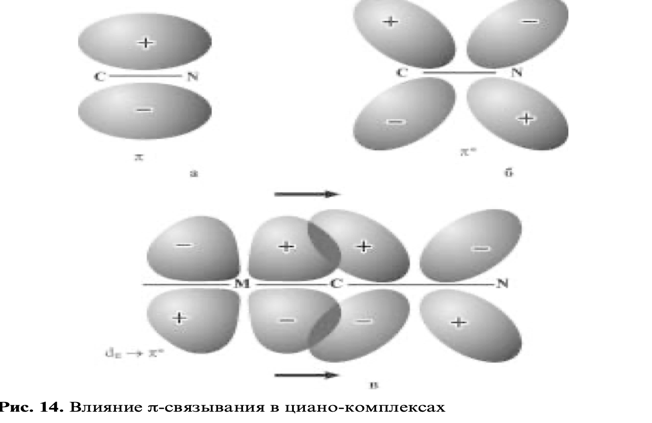
\includegraphics[scale=1.00]{images/L-M-pi2.png}
\end{figure}